\documentclass[../manuale-sviluppatore.tex]{subfiles}

\begin{document}
\subsection{Visione generale}%
\label{subs:installazione_applicazione_di_addestramento}
Il programma di addestramento è costituito da un'applicazione web che si basa su NodeJS e sul framework Electron.
Tale applicazione effettua l'addestramento su un dataset importato dall'utente attraverso un file CSV, attraverso un algoritmo di predizione da lui scelto tra quelli disponibili, per poi produrre in output
un file JSON contenente la definizione del predittore.
All'interno dell'applicazione è stato utilizzato il design pattern architetturale Model-View-controller per gestire gli aspetti fondamentali dell'applicazione perché esso fornisce i seguenti vantaggi:
\begin{itemize}
    \item Rende le componenti indipendenti e permette una suddivisione del lavoro migliore;
    \item Rende l'applicazione facilmente scalabile nel caso si dovessero creare nuove view e i controller ad esse associati, o nel caso di aggiunta di nuovi funzionalità relative a una delle 3 classi attuali del MVC;
    \item Permette di avere un controllore separato dal resto dell’applicazione, il che rende la progettazione più semplice e permette di concentrare gli sforzi sulla logica del funzionamento dell'applicazione.
\end{itemize}

È stato poi usato il design pattern Object Adapter per la gestione delle diverse librerie di algoritmi di predizione perché esso fornisce i seguenti vantaggi:
\begin{itemize}
    \item Facilita la conversione delle interfacce delle diverse librerie di algoritmi di predizione dei dati;
    \item Permette di riutilizzare librerie di algoritmi già esistenti pensando solo a come adattarle al modello dei dati;
    \item Permette di estendere facilmente l'applicazione nel caso di aggiunta di nuovi algoritmi di predizione.
\end{itemize}

\begin{figure}[H]
   \begin{center}
        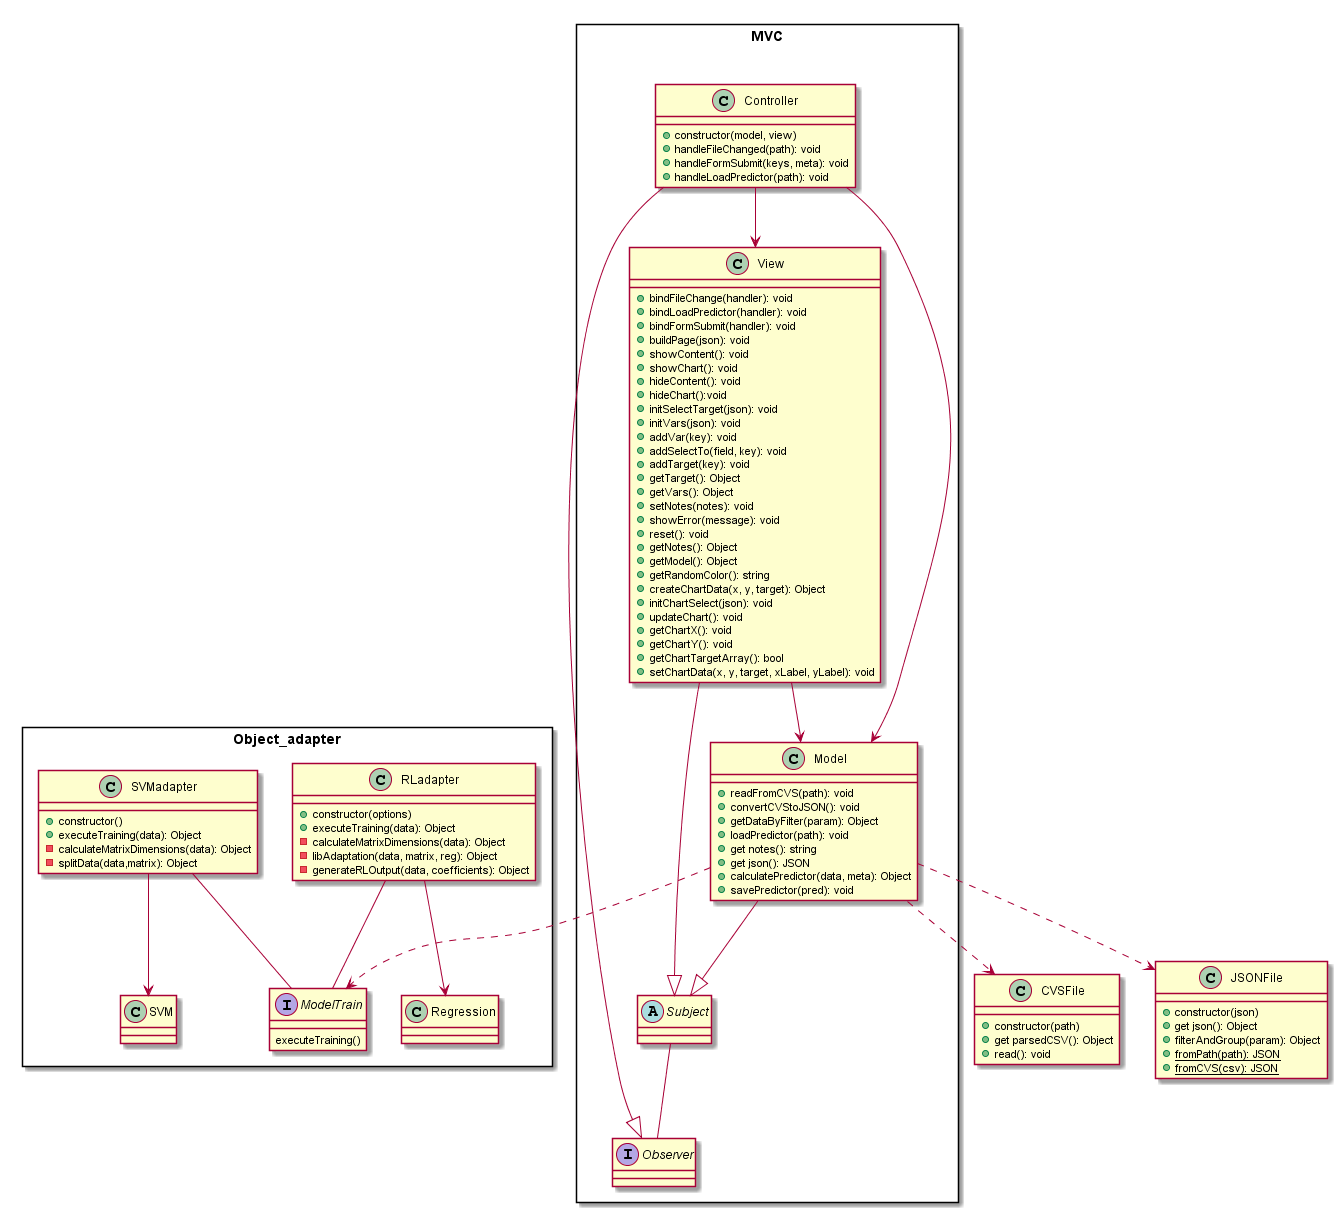
\includegraphics[width=15cm]{img/classDiagramTA.png}
        \caption{Diagramma delle classi - addestramento}
        \label{fig:diagramma_classi}
    \end{center}
\end{figure}

\begin{figure}[H]
    \begin{center}
         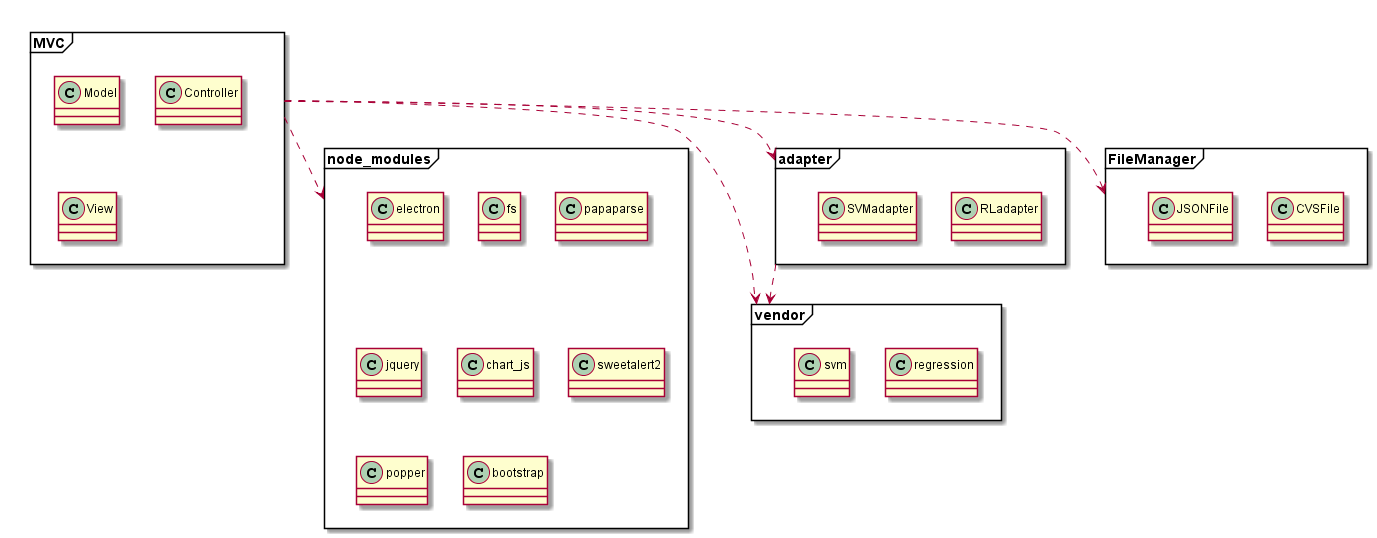
\includegraphics[width=10cm]{img/packagesDiagramTA.png}
         \caption{Diagramma dei package - addestramento}
         \label{fig:daa}
     \end{center}
 \end{figure}



\subsection{Design pattern - MVC}
\label{ssec:design_pattern_mvc}
Il design MVC è stato implementato realizzando le tre classi principali: Model, View e Controller per gestire i tre aspetti fondamentali dell'applicazione.
La classe View gestisce l'interfaccia grafica della classe, gestendo quindi anche le interazioni con il framework Electron utilizzato dal gruppo.
La classe Model gestisce i dati che l'utente carica attraverso il file CVS o attraverso un predittore già allenato. Tale classe per gestire i due diversi tipi di file interagisce con le classi
CVSFile che gestisce i file di tipo CVS, quindi il file caricato inizialmente dall'utente, e JSONFile che gestisce i predittori che sono file di tipo JSON.
La classe Controller gestisce gli eventi e le interazioni tra l'interfaccia grafica e il modello dei dati, permettendo di eseguire semplici richieste richiamando funzioni delle due rispettive classi.

\begin{figure}[H]
    \begin{center}
         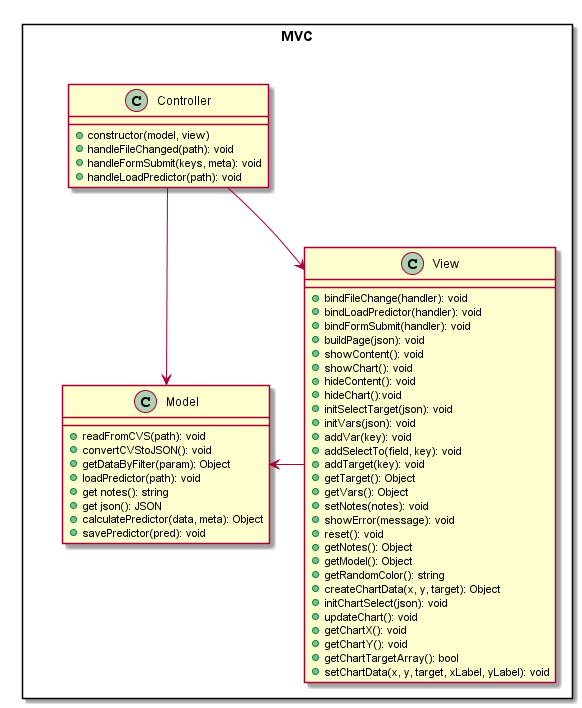
\includegraphics[width=9cm]{img/mvcTA.png}
         \caption{Implementazione MVC - addestramento}
         \label{fig:MVC}
     \end{center}
 \end{figure}

\subsection{Design pattern - Object Adapter}
\label{ssec:design_pattern_object_adapter}
Per gestire le diverse librerie esterne che implementano gli algoritmi di Regressione lineare e Support vector machine è stato utilizzato il design pattern Object Adapter.
Pur non essendo possibile con node.js implementare un'interfaccia nativa, è stata creata la classe modelTrain, utilizzata come interfaccia, che lancia un'eccezione nel caso
in cui le sottoclassi adapter che estendono l'interfaccia, non implementino il metodo executeTraining(data).
Seguendo questo principio sono state create le classi RLadapter e SVMadapter che estendono l'interfaccia modelTrain e implementano il metodo ad essa associato, oltre a vari metodi privati
utilizzati per rendere il codice più leggibile e funzionale.
Le due classi adapter hanno anche un riferimento all'oggetto della libreria dell'algoritmo che intendono adattare, quindi SVMadapter ha un riferimento dell'oggetto della libreria svm e
RLadapter avrà come riferimento l'oggetto della libreria regression. Tali riferimento saranno utilizzati per richiamare i metodi delle librerie all'interno del metodo executeTraining(data)
e, se necessario, anche nei metodi privati della classe.

\begin{figure}[H]
    \begin{center}
         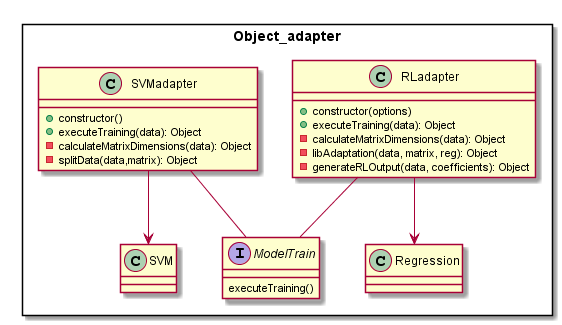
\includegraphics[width=9cm]{img/objectAdapterTA.png}
         \caption{Implementazione Object Adapter - addestramento}
         \label{fig:object_adapter}
     \end{center}
 \end{figure}

\subsection{Addestramento dei dati senza predittore}
\label{ssec:addestramento_dati_senza_predittore}
Una volta avviata l'applicazione l'utente inserisce il file CSV contenente i dati per l'addestramento, in quel momento nella View scatta l'evento relativo all'inserimento del file
che attiva Controller tramite handle(path) in cui viene passato il percorso del file selezionato dall'utente. Il Controller quindi riceve questo segnale dalla View, interagisce col Model
per leggere i dati dal file e salvarli in un oggetto CVSFile, una volta salvati il Controller riceve l'avvenuto salvataggio dei dati rimanda alla View le informazioni necessarie per eseguire
la funzione buildPage() che inserisce all'interno dell'interfaccia la form per selezionare il modello di predizione dei dati, il grafico iniziale e le varie label per selezionare quali variabili
visualizzare e salvare nel futuro predittore. \\
Quando l'interfaccia è pronta, l'utente seleziona il tipo di modello (ossia l'algoritmo di predizione) per il quale intende allenare i dati inseriti, non appena viene selezionato uno dei modelli
presenti nei radiobox, la View registra attraverso un evento la scelta del modello e al suo interno richiama la funzione updateChart() per ridisegnare il grafico secondo le esigenze di quel modello.
Successivamente l'utente può scegliere quali variabili visualizzare sul grafico, che viene aggiornato simultaneamente, e una volta che nella form di submit sceglie le variabili da inserire nel predittore e la variabile target,
quando viene premuto il pulsante submit inizia la parte di predizione e creazione del predittore. \\
La View riconosce la pressione del pulsante, fa gli opportuni controlli sulle variabili selezionate e trasmette attraverso handler(data,meta) le informazioni al Controller per iniziare l'addestramento reale.
attraverso l'handler della View il controller attiva la funzione handleFormSubmit(keys,meta) che si occupa di filtrare i dati all'interno del modello, in base alle variabili selezionate, per poi riceve le variabili filtrate dal Model.
Una volta ottenuti i dati filtrati il controller richiama la funzione calculatePredictor(data,meta) del Model che, in base all'algoritmo scelto, crea o un'istanza della classe RLadapter o un'istanza della classe SVMadapter, in quella classe verrà eseguito il metodo di training sui dati filtrati.
Al termine dell'allenamento il model riceve i dati della predizione e aggiunge le note e il tipo di modello di addestramento a tali dati creando il predittore. \\
Alla fine il controller richiama la funzione savePredictor(pred) che richiama indirettamente la funzione di save di ipcRender per salvare il file nel computer dell'utente.

\begin{figure}[H]
    \begin{center}
         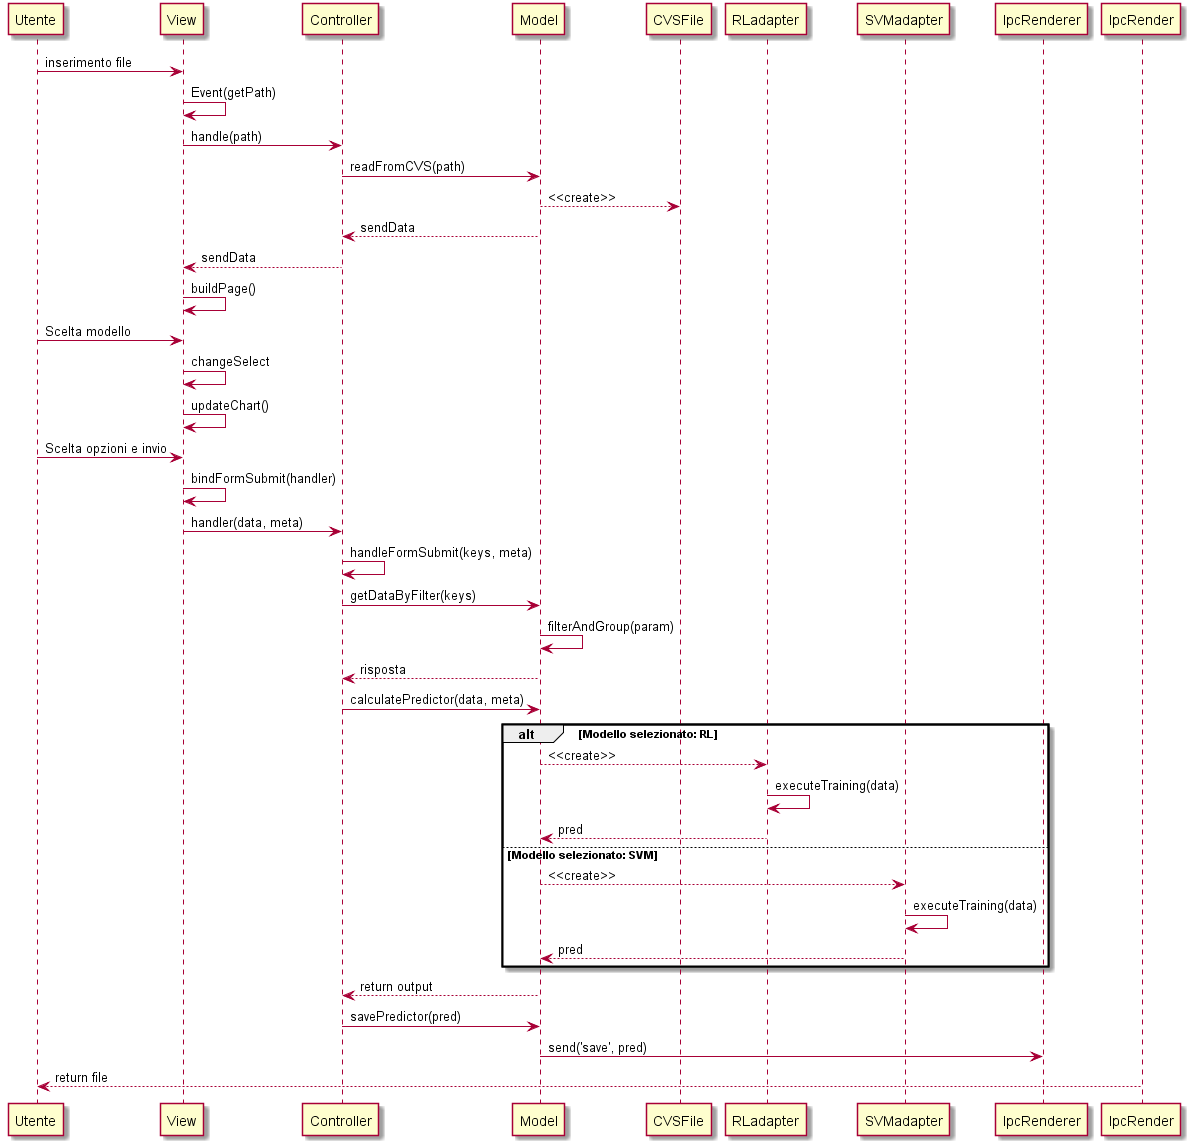
\includegraphics[width=13cm]{img/sequenceDiagramNoP.png}
         \caption{Diagramma di sequenza - Addestramento senza predittore}
         \label{fig:diagramma_di_sequenza}
     \end{center}
 \end{figure}

\subsection{Addestramento dei dati con predittore}
\label{ssec:addestramento_dati_con_predittore}
L'addestramento con l'inserimento del predittore aggiunge al workflow la parte di inserimento di un predittore.
Quando l'utente inserisce il predittore viene scaturito un evento nella View che ottiene il percorso del file predittore e attraverso handler(path) lo passa al Controller,
che richiama il metodo loadPredictor(path) del Model per creare l'oggetto JSONFile per salvare il file predittore.
Una volta caricato il file nell'oggetto il Model richiede le note presenti nel predittore e le restituisce al Controller che provvederà a mandarle alle View in modo da settare le proprie impostazioni con le preferenze presenti nel predittore.

\begin{figure}[H]
    \begin{center}
         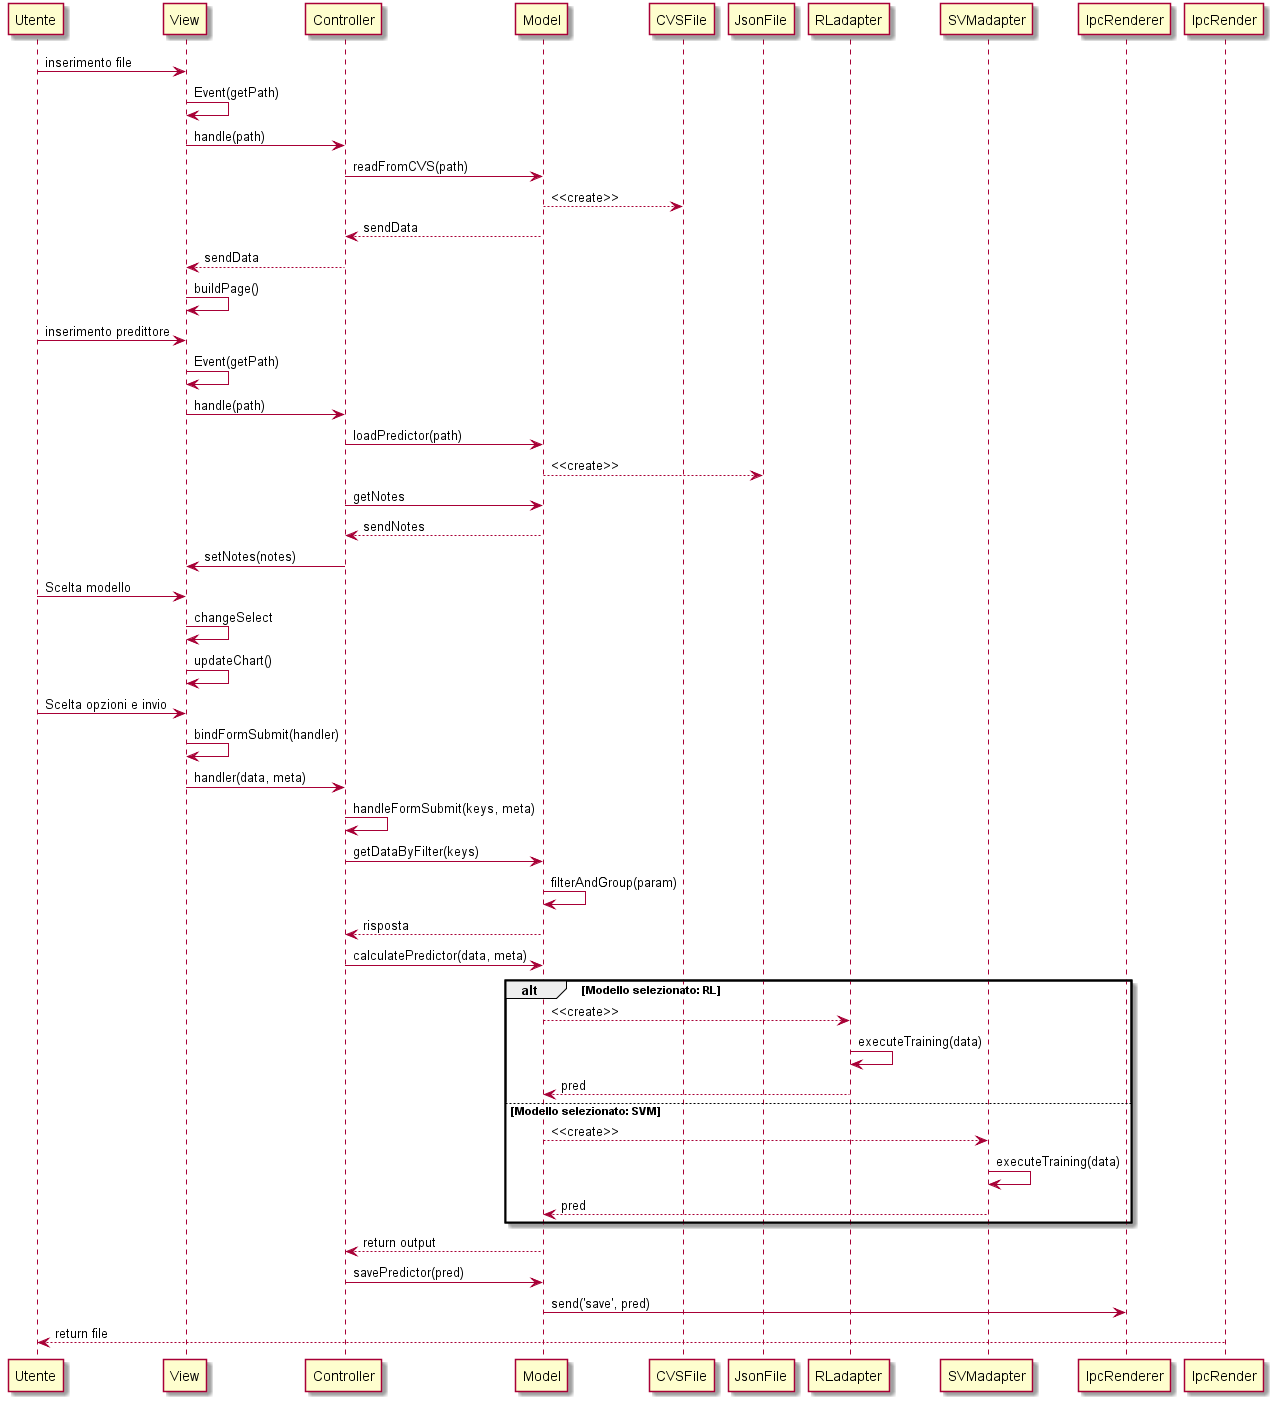
\includegraphics[width=13cm]{img/sequenceDiagramConP.png}
         \caption{Diagramma di sequenza - Addestramento con predittore}
         \label{fig:daa}
     \end{center}
 \end{figure}

\end{document}
